\section{DRL}
\begin{frame}{Deep Reinforcement Learning (DRL) Model}
    \centering
    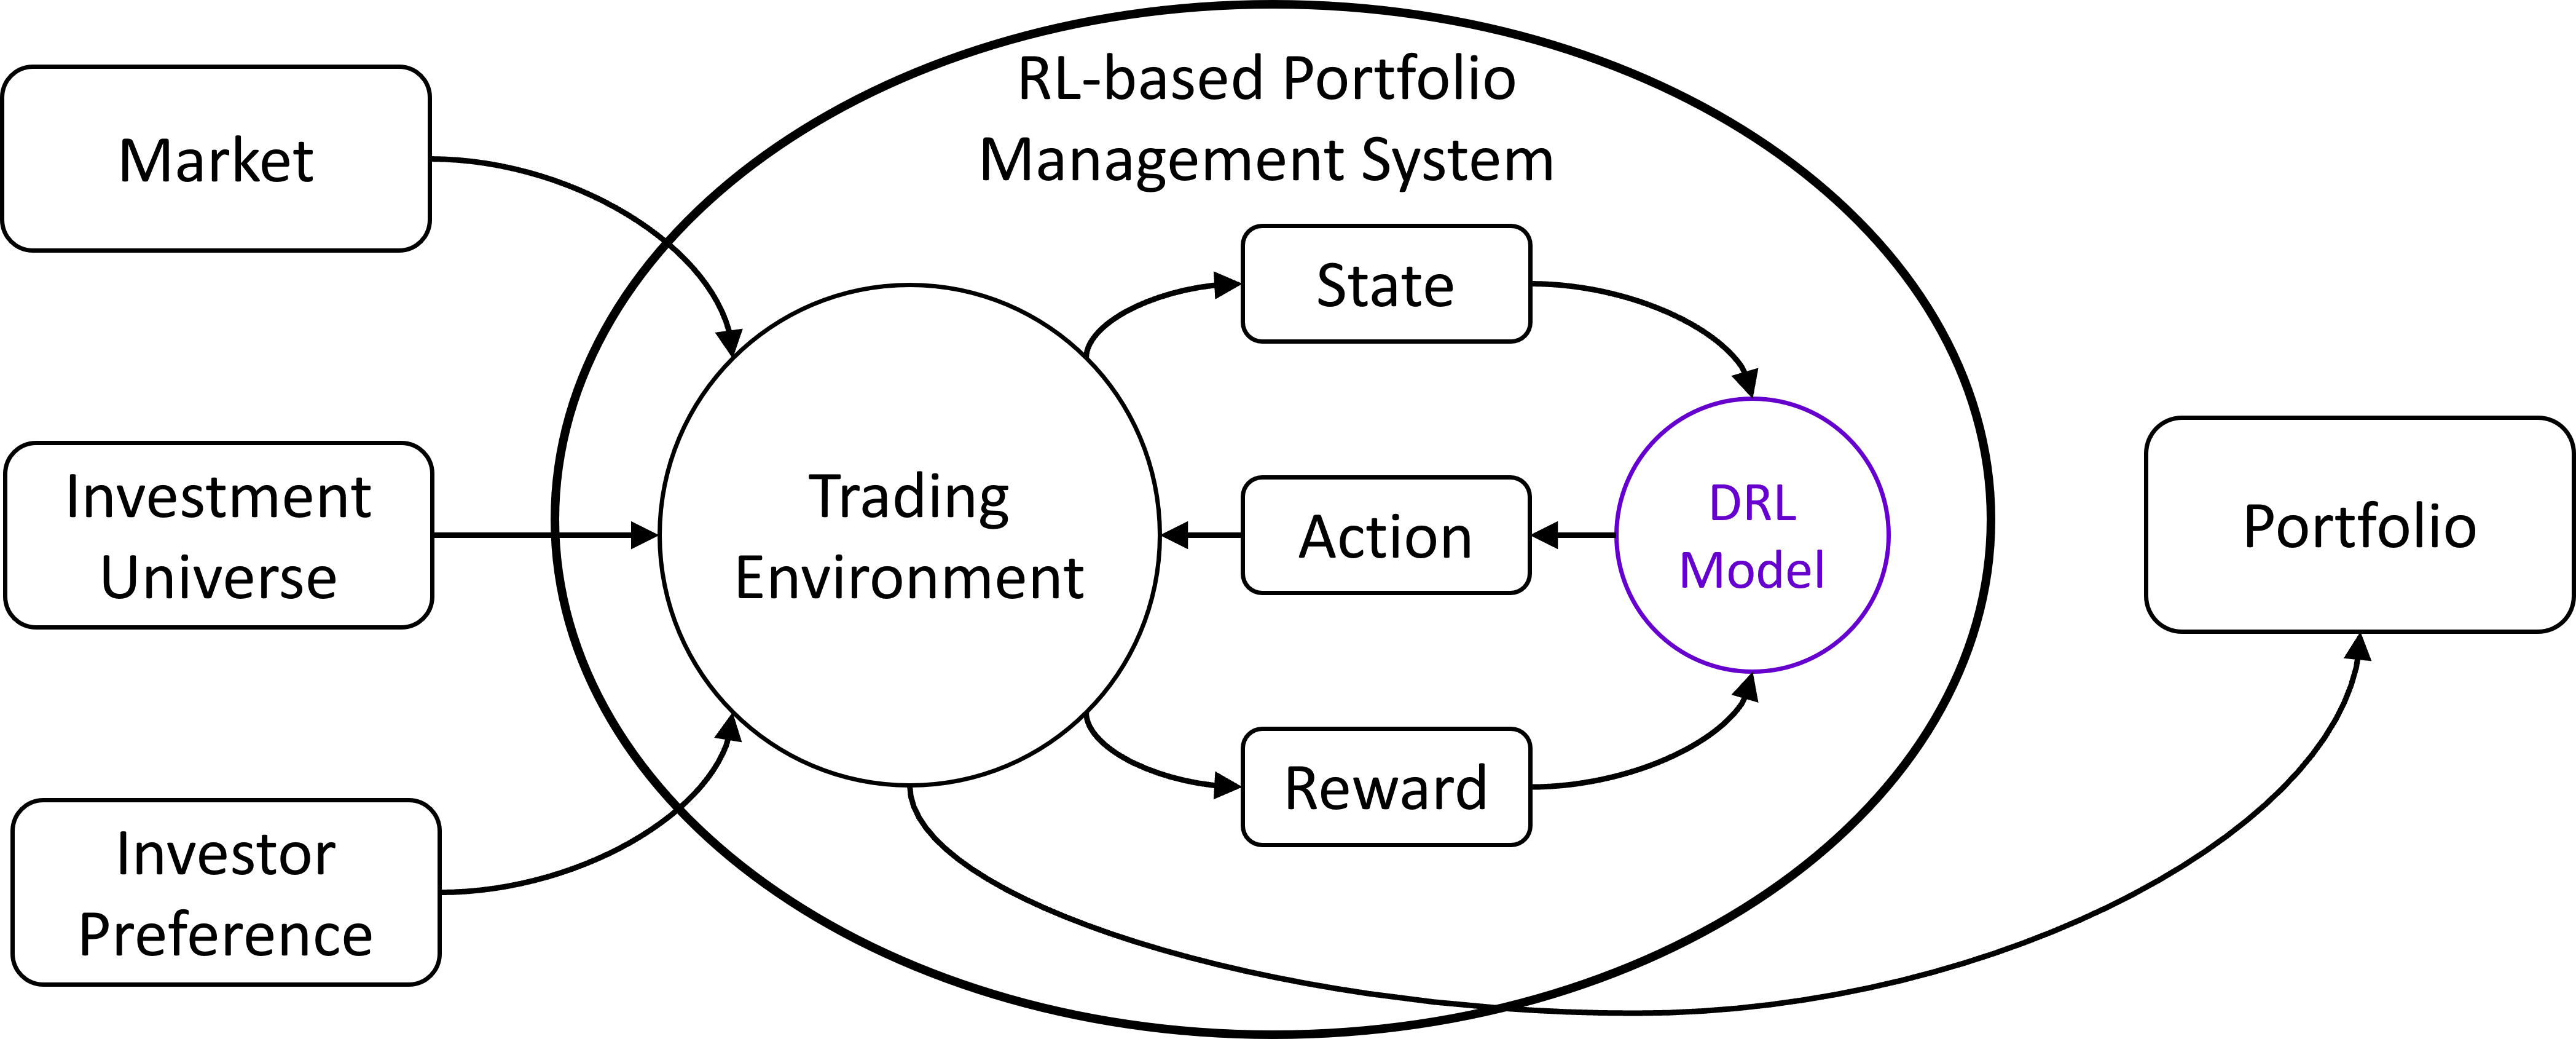
\includegraphics[width=10cm]{images/drl_model.png}
\end{frame}

\begin{frame}{Reinforcement Learning}
    \centering
    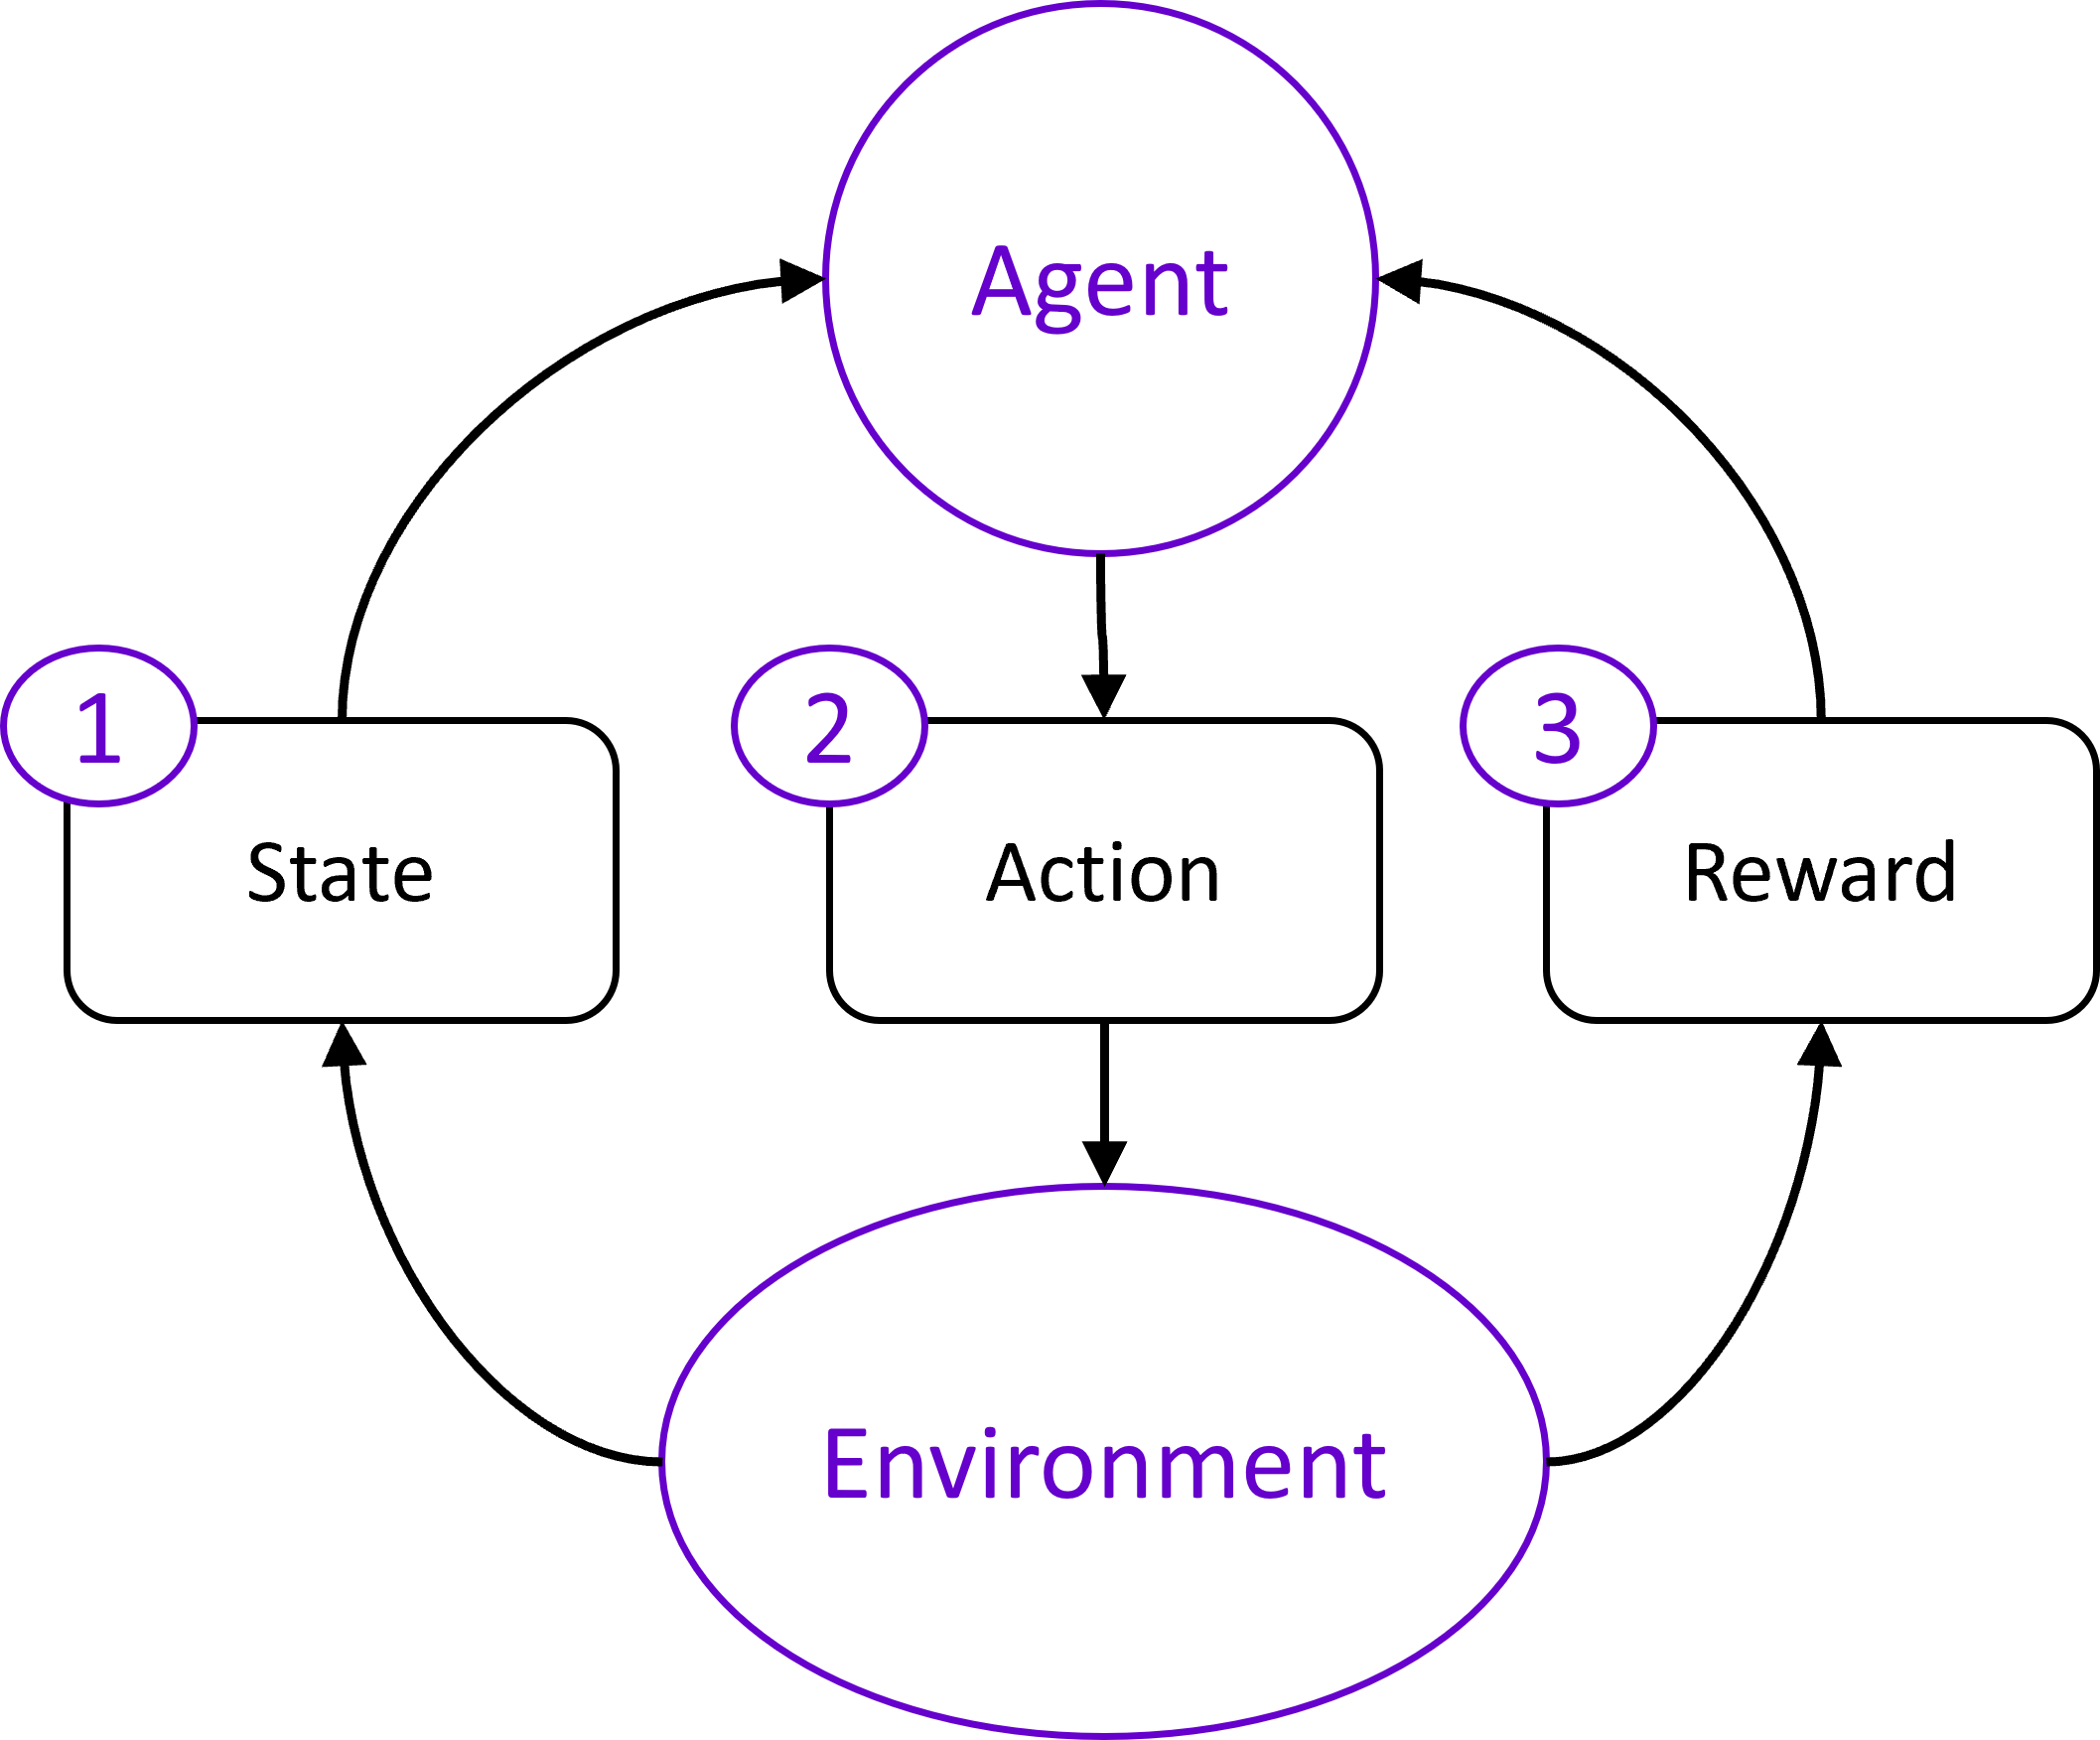
\includegraphics[width=8cm]{images/rl_overview.png}
\end{frame}



\begin{frame}{Value Optimization vs Policy Optimization}
\end{frame}

\begin{frame}{On-Policy vs Off-Policy}
\end{frame}

\begin{frame}{Comparison}
\end{frame}


\begin{frame}{Determinisitc Policy vs Stochastic Policy}
\end{frame}

\subsection{Soft Actor-Critic}
\begin{frame}{Actor-Critic}
    \centering
    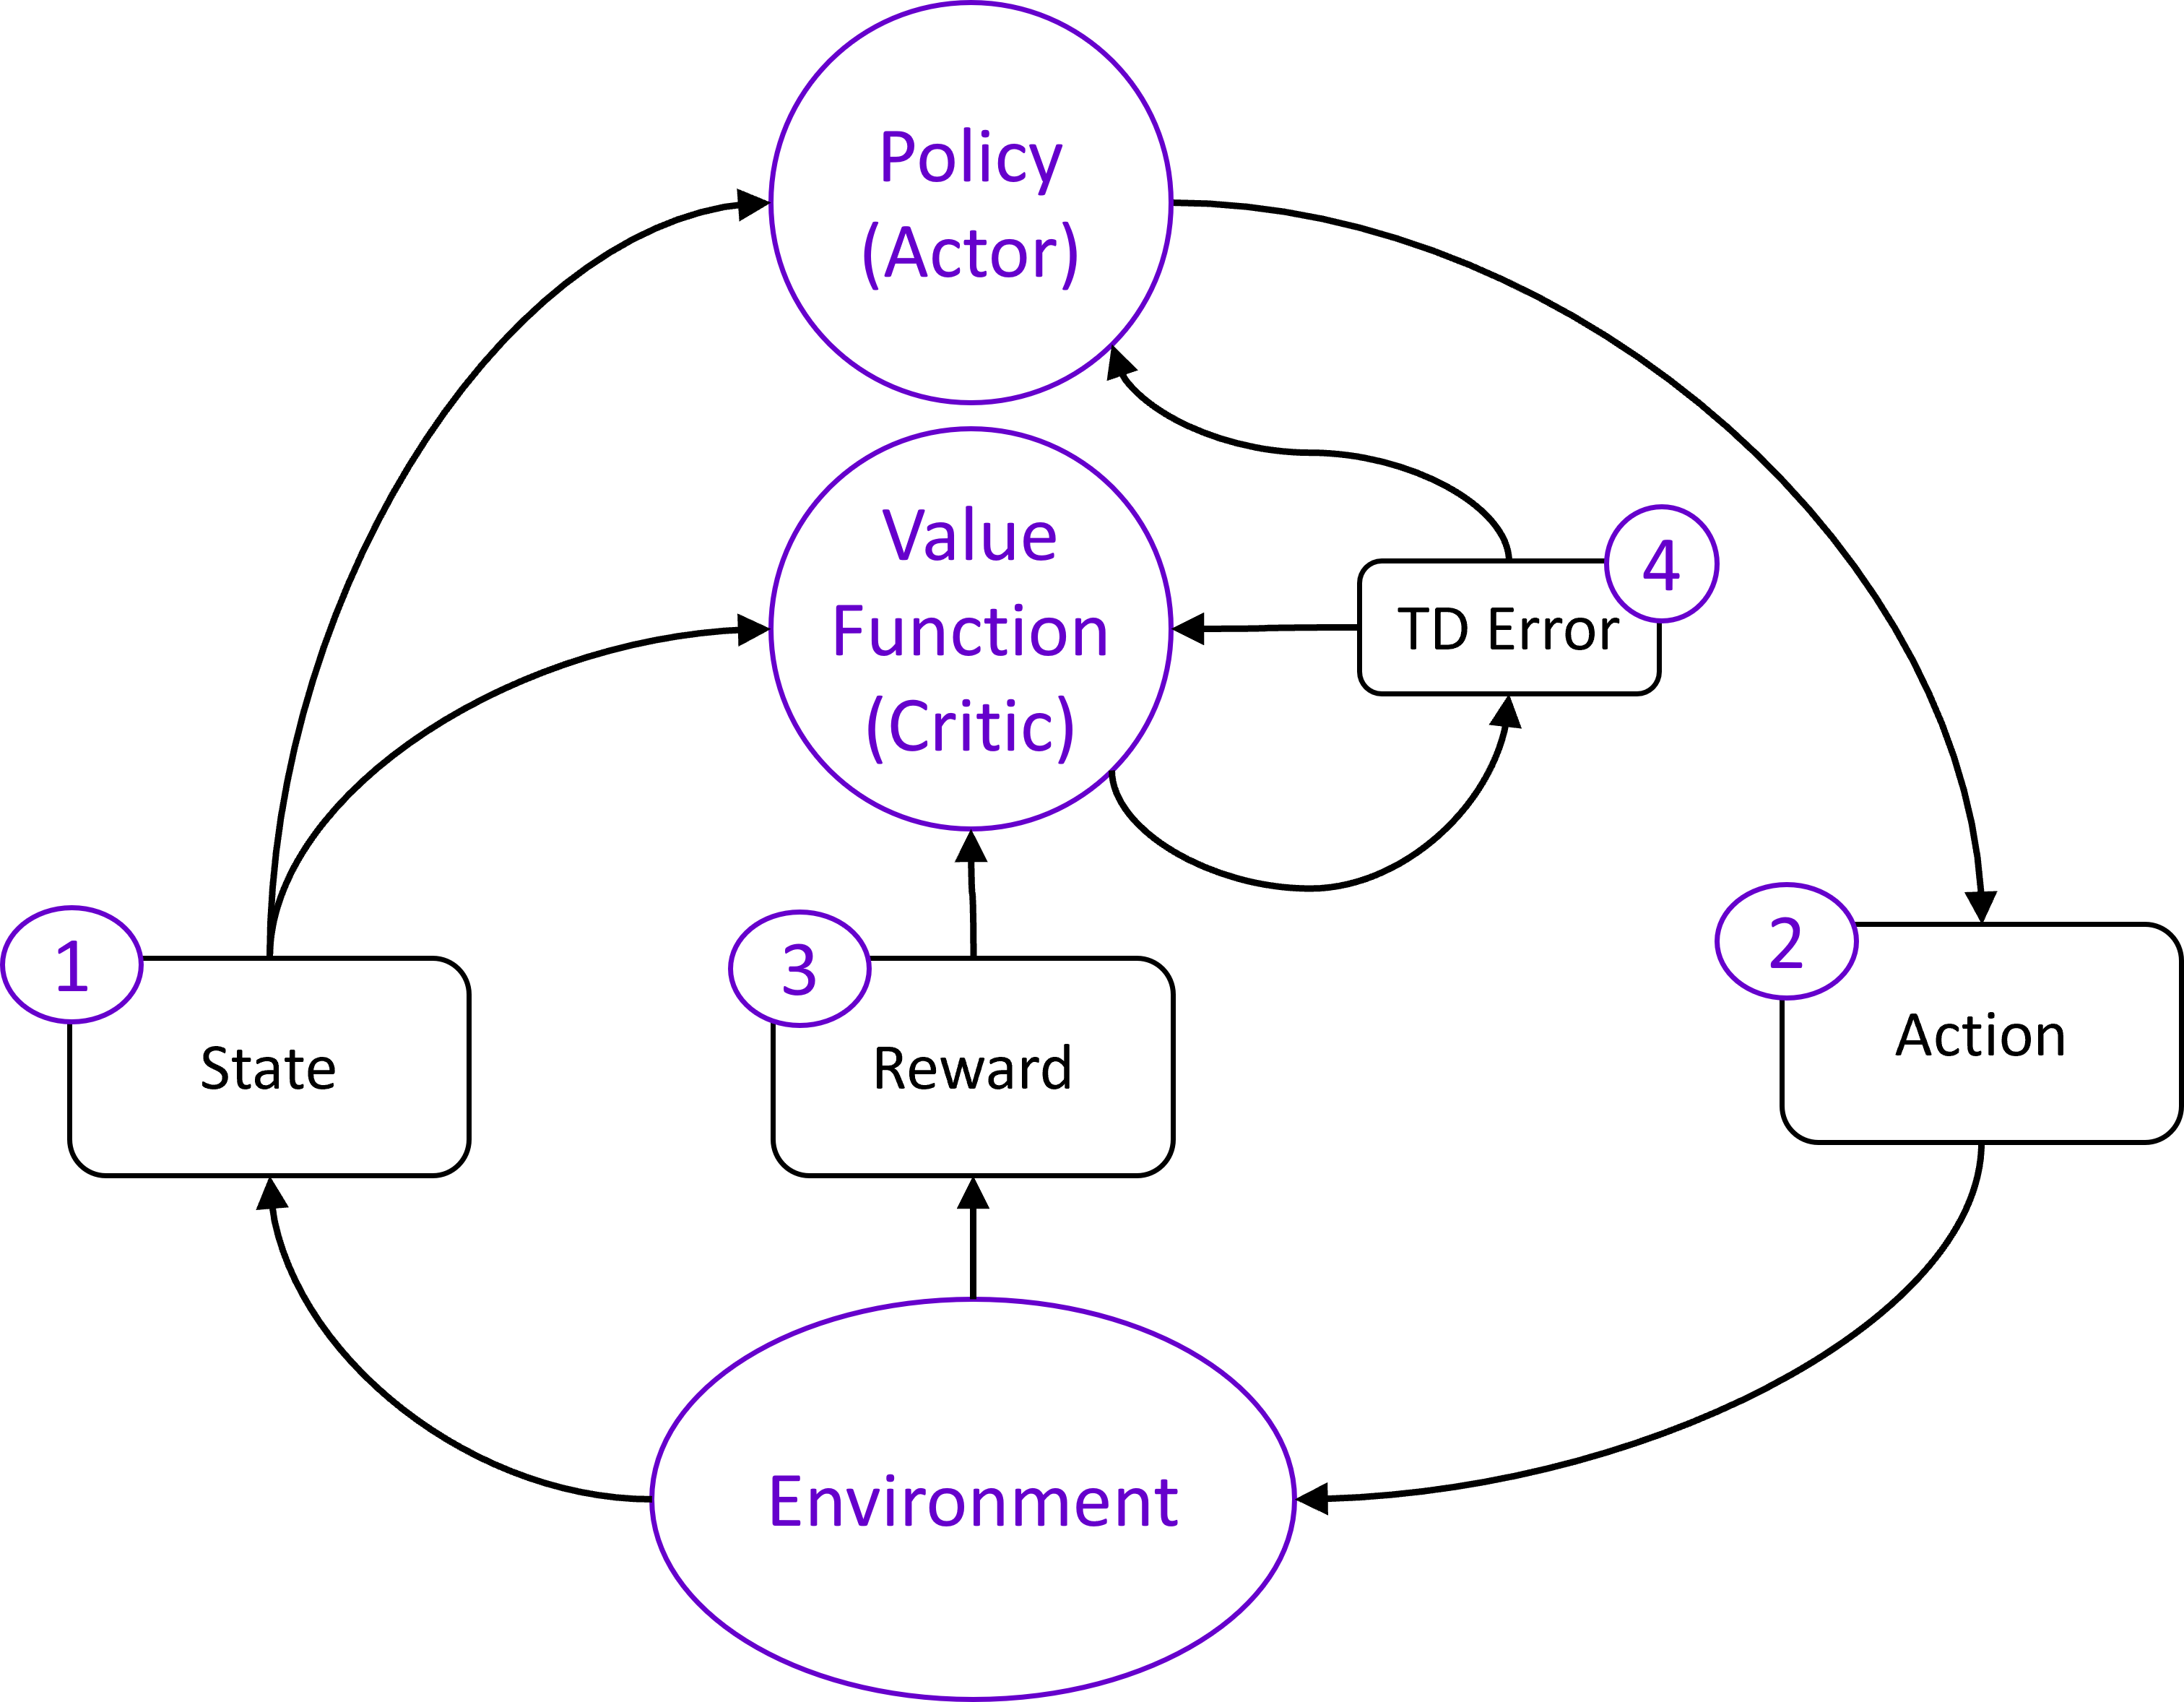
\includegraphics[width=8cm]{images/actor_critic.png}
\end{frame}

\begin{frame}{Soft Actor-Critic}
We Use Soft Actor-Critic (SAC), as the RL model.
\begin{block}{SAC Overview}
\begin{itemize}
    \item Optimizes a stochastic policy in an off-policy way
    \item Optimizes the policy with \alert{entropy regularization} and takes entropy, measuring randomness in the policy, into account.
\end{itemize}
\end{block}
\begin{alertblock}{Reward Scale}
SAC is highly sensitive to the scaling of the reward. 
\begin{itemize}
    \item If reward scale is too small, the reward will fail to affect the model, and the policy will become nearly uniform.
    \item If reward scale is too large, the model will learn quickly and become deterministic, leaving no room for exploration.
\end{itemize}
\end{alertblock}
\end{frame}